\subsubsection{Description}
%Describe your concept of the HVD and how it can be operated.

A circular connector ASHD 0 24-44420 S N + ASHD 6 24-44420 P N is used as HVD. By disconnecting HVD positive and negative pole of Tractive System is quickly disconnected. Disconnection is done by turning the plug left, this motion is clearly hinted by a label. By turning left the lever system in connector disconnect pins and release plug. There are sockets used in the receptacle rather than pins, therefore no harm can be done to crew by touching the receptacle. 

Interlock is achieved by using ASHD 0 24-44420 S N - 016 as a receptacle and ASHD 6 24-44420 P N - 016 as plug. This connector has several other low current pins size AWG 22. Two of them are used as interlock, there is only shunt loop at the plug.

Datasheet is to be seen in \ref{app:HVD}.

\subsubsection{Wiring, cables, current calculations, connectors}
%Describe wiring, show schematics, describe connectors and cables and show useful data regarding the wiring.  Include information on the working voltage and current rating of the HVD.

HVD is placed between Accumulator Pack and Motor Controllers, Energy Meter is also placed after Motor Controller in the circuit. Positive pole of Tractive system is interrupted. There are four pins connected to each other in the plug and the back of the plug is sealed. OLFLEX HEAT 180 SiF are used as HV wires, four pins are used. One HV pin is rated to 200A.

\subsubsection{Position in car}
%Provide CAD-renderings showing all relevant parts. Mark the parts in the rendering, if necessary.

HVD is placed on panel next to Maser switches and Measure points, see \ref{fig:hvd-position}.

\begin{figure}[H]
	\centering
	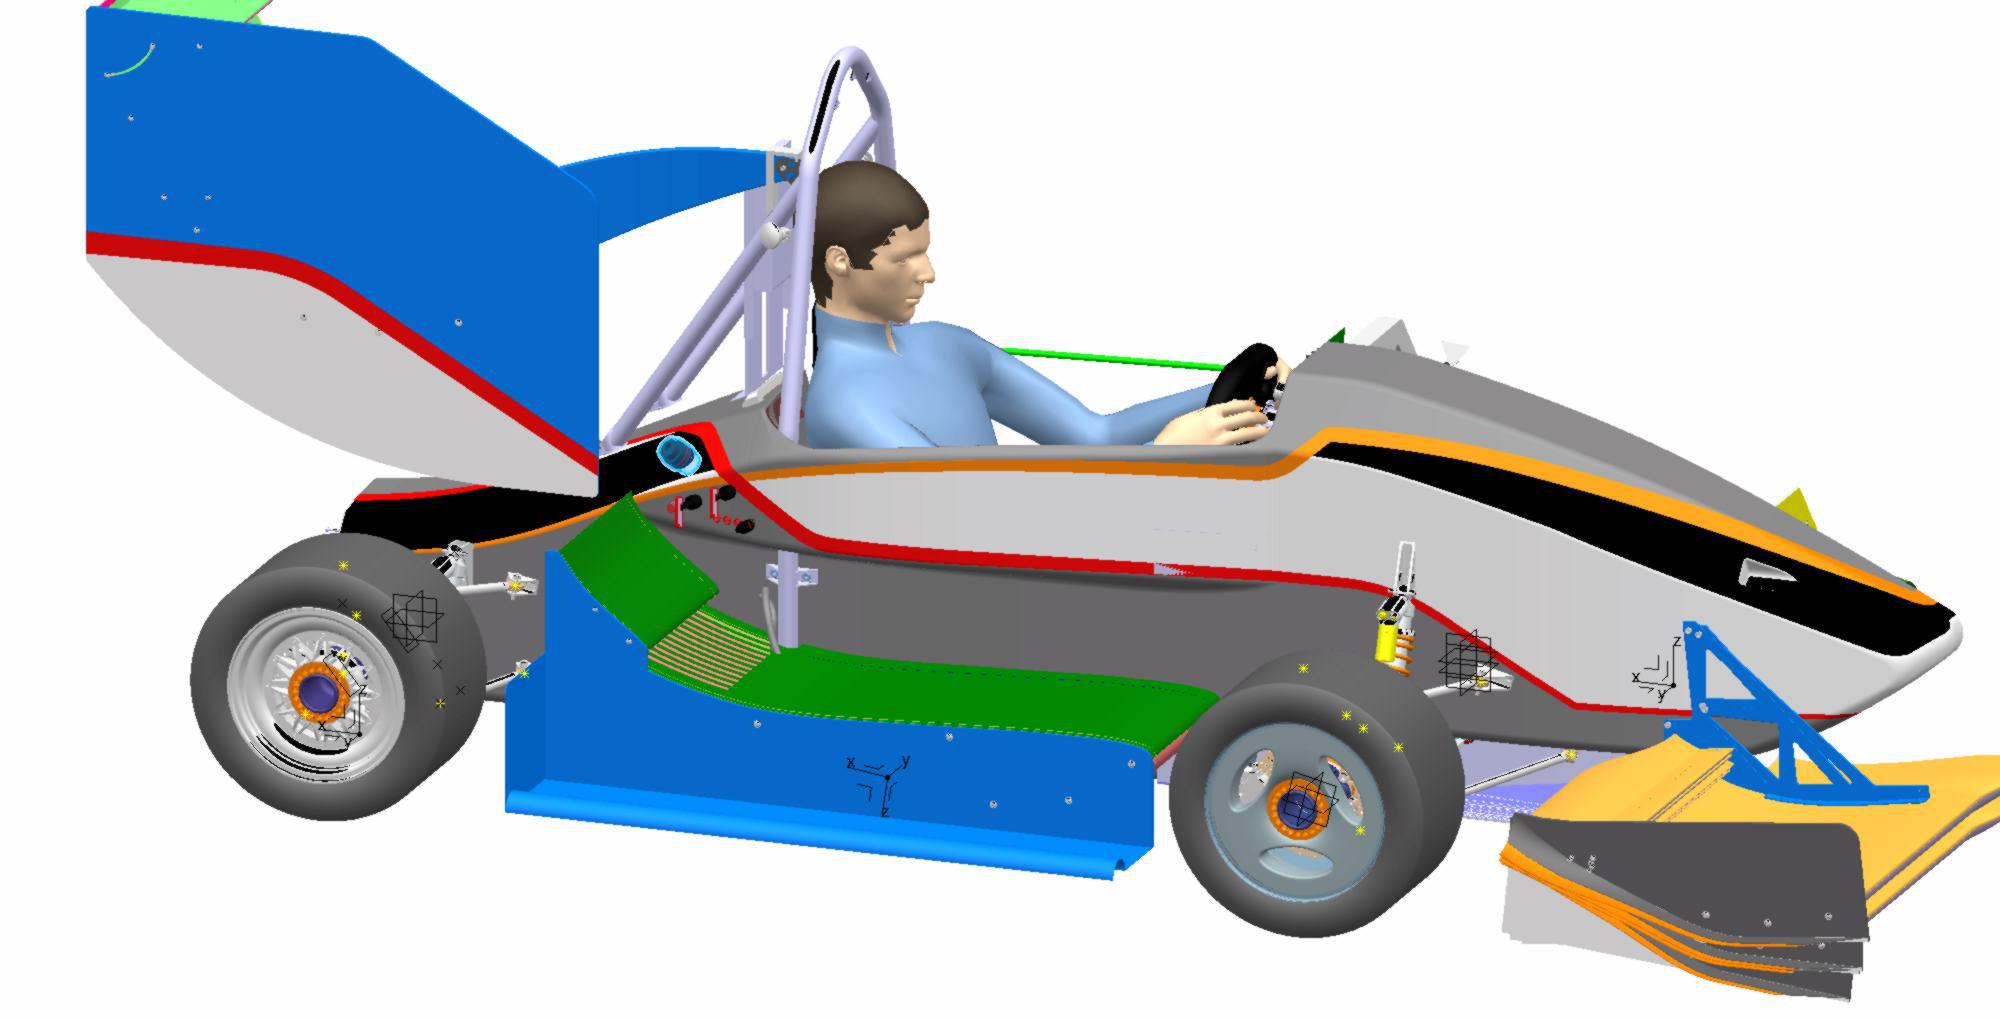
\includegraphics[width=\textwidth,trim={15cm 2cm 15cm 5cm},clip]{./img/hvd-position.jpg}
	\caption{HVD position.}
	\label{fig:hvd-position}
\end{figure}